

\begin{frame}{Continuons la conception\,: les séjours}

Etudions l'association ``un voyageur séjourne dans un logement''

\vfill

\begin{center}
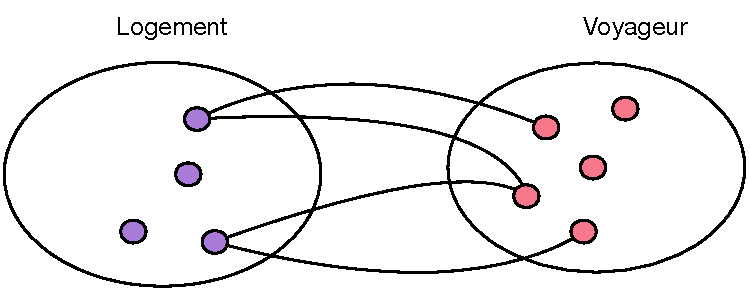
\includegraphics[width=8cm]{../figures-sql/graphe-sejours}
\end{center}
\vfill

Décisions à prendre:

\begin{redbullet}
  \item Certains voyageurs peuvent-ils séjourner dans plusieurs logements\,?
    \item Un logement peut-il recevoir plusieurs voyageurs\,?
\end{redbullet}

\end{frame}


\begin{frame}{Associations plusieurs-à-plusieurs}

Ajout  de l'association représentant les séjours.

\vfill

\begin{center}
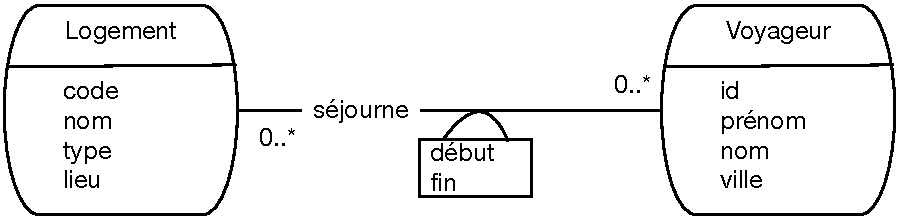
\includegraphics[width=10cm]{../figures-sql/association-sejour}
\end{center}

\vfill

Une association est identifiée par les deux entités qu'elle lie, et donc par
la paire (codeLogement, idVoyageur).

\vfill

Aie, un  même voyageur séjourne \alert{au plus} une fois dans un logement\,?

\end{frame}

%%%%%%%%
\begin{frame}{Réification des associations plusieurs-à-plusieurs}

On peut \alert{remplacer} une association plusieurs-à-plusieurs par une \alert{entité}
et des associations un-à-plusieurs.
\vfill

\begin{center}
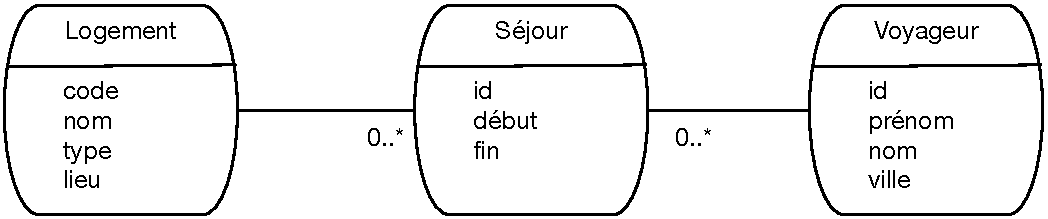
\includegraphics[width=11cm]{../figures-sql/association-sejour-reifiee}
\end{center}

\vfill
Souvent un bon choix: il est plus facile d'exprimer des contraintes sur une entité
que sur une association.
\end{frame}
%%%%%%ù


\begin{frame}{Entités faibles}

Identification d'une entité \alert{relativement} à une autre entité (toujours
un-à-plusieurs).

\vfill


\includegraphics[width=9cm]{../figures-sql/faible}

\vfill

Définit une DF $codeLogement, codeActivit\acute{e} \to description$
\end{frame}

\begin{frame}{À retenir}

Le modèle entité association
\vfill
\begin{redbullet}
  \item Entité: objets autonomes, identifiables, persistants.
 \item Associations: liens entre entités, caractérisées par des \alert{cardinalités}
 \item On peut toujours se ramener à des associations un-à-plusieurs.
 \item Quelques subtilités peuvent être utiles... 
\end{redbullet}

\vfill

Vous savez (presque) tout. La mise en {\oe}uvre est une
question de pratique et d'expérience

\end{frame}

